\documentclass[11pt]{scrartcl}
\usepackage{polski}
\usepackage[polish]{babel}

\usepackage{graphicx, float, caption, subcaption, amsmath}
\usepackage{tabularx, multirow, hyperref, enumitem, listings}
\usepackage{xcolor}
%\usepackage{minted}

\hypersetup{
    colorlinks=true,
    linkcolor=black,
    urlcolor=black,
    citecolor=black
}

\definecolor{md-black}{rgb}{0.12, 0.12, 0.12}
\definecolor{md-teal}{rgb}{0.38, 0.79, 0.69}
\definecolor{md-mauve}{rgb}{0.76, 0.52, 0.75}
\definecolor{md-yellow}{rgb}{0.86, 0.86, 0.67}
\definecolor{md-green}{rgb}{0.13, 0.55, 0.13}
\definecolor{md-red}{rgb}{0.82, 0.10, 0.14}
\definecolor{md-purple}{rgb}{0.69, 0.33, 0.73}
\definecolor{md-orange}{rgb}{0.96, 0.42, 0.18}
\definecolor{md-gray}{rgb}{0.44, 0.46, 0.51}
\lstset{
    language=Python,
    basicstyle=\color{md-teal}\ttfamily,
    keywordstyle=\color{md-mauve},
    commentstyle=\color{md-green},
    stringstyle=\color{md-red},
    numbers=left,
    numberstyle=\small\color{md-gray}\ttfamily,
    stepnumber=1,
    numbersep=5pt,
    backgroundcolor=\color{md-black},
    showspaces=false,
    showstringspaces=false,
    showtabs=false,
    frame=none,
    tabsize=4,
    captionpos=b,
    breaklines=true,
    breakatwhitespace=false,
    escapeinside={\%*}{*)},
    numbersep=-10pt,
    morekeywords={as},
    classoffset=1,
    morekeywords={quad},
    keywordstyle=\color{md-yellow},
    classoffset=0
}

\graphicspath{{images/}}

\title{Laboratorium 5 - Aproksymacja}
\author{Mateusz Podmokły - II rok Informatyka WI}
\date{4 kwiecień 2024}

\begin{document}
    \maketitle
    \section{Treść zadania}
    \textbf{Zadanie 1.} Wykonaj aproksymację średniokwadratową
    punktową populacji Stanów Zjednoczonych w przedziale
    $[1900,1980]$ wielomianami stopnia $m$ dla $0 \leq m \leq 6$. \\
    Dla każdego $m$ dokonaj ekstrapolacji wielomianu do roku 1990.
    Porównaj otrzymaną wartość z prawdziwą wartością dla roku 1990
    wynoszącą 248 709 873. \\
    Wyznacz optymalny stopień wielomianu za pomocą kryterium
    informacyjnego Akaikego (ang. Akaike information criterion):
    \[
        AIC=2k+nln \left( \frac{\sum_{i=1}^{n}[y_i-\hat{y}(x_i)]^2}
        {n} \right),
    \]
    gdzie $y_i$ $(i=1, \ldots ,n)$ oznacza prawdziwą liczbę osób
    w roku $x_i$, $k$ to liczba parametrów wielomianu ($k=m+1$),
    natomiast $\hat{y}(x_i)$ liczbę osób przewidywaną przez model,
    tzn. wartość wielomianu $\hat{y}(x)$. Ponieważ rozmiar próbki
    jest niewielki (dane z dziewięciu lat, $n-9$), $\frac{n}{k}<40$,
    należy użyć wzoru ze składnikiem korygującym:
    \[
        AIC_c=AIC+\frac{2k(k+1)}{n-k-1}
    \]
    Mniejsze wartości kryterium Akaikego oznaczają lepszy model.

    \subsection*{}
    \textbf{Zadanie 2.} Wykonaj aproksymację średniokwadratową ciągłą
    funkcji $f(x)=\sqrt{x}$ w przedziale $[0,2]$ wielomianem drugiego
    stopnia, używając wielomianów Czebyszewa.

    \section{Specyfikacja użytego środowiska}
    Specyfikacja:

    \begin{itemize}
        \item Środowisko: Visual Studio Code,
        \item Język programowania: Python,
        \item System operacyjny: Microsoft Windows 11,
        \item Architektura systemu: x64.
    \end{itemize}

    \section{Rozwiązanie problemu}
    \subsection{Biblioteki}
    W realizacji rozwiązania wykorzystane zostały następujące
    biblioteki:
    \begin{lstlisting}
        import numpy as np
        import matplotlib.pyplot as plt
        from scipy.integrate import quad
    \end{lstlisting}

    \subsection{Zadanie 1.}
    Mamy $n$ punktów, dla których chcemy wyznaczyć wielomian
    aproksymacyjny stopnia $m$. Aby wyznaczyć współczynniki wielomianu
    obliczamy macierz
    \[
        A=
        \begin{bmatrix}
            1 & x_0 & x_0^2 & \cdots & x_0^m \\
            1 & x_1 & x_1^2 & \cdots & x_1^m \\
            \vdots & \vdots & \vdots & \ddots & \vdots \\
            1 & x_n & x_n^2 & \cdots & x_n^m
        \end{bmatrix}
    \]
    Przyjmujemy
    \[
        y=
        \begin{bmatrix}
            f(x_0) \\
            f(x_1) \\
            \vdots \\
            f(x_n)
        \end{bmatrix}
    \]
    oraz jako wektor współczynników
    \[
        c=
        \begin{bmatrix}
            c_0 \\
            c_1 \\
            \vdots \\
            c_m
        \end{bmatrix}
    \]
    Obliczamy $c$ z równania normalnego:
    \[
        A^TAc=A^Ty
    \]
    \[
        c=(A^TA)^{-1}A^Ty
    \]
    Otrzymujemy wielomian aproksymacyjny postaci
    \[
        p(x)=\sum_{j=0}^{n}c_jx^j
    \]

    \subsection{Zadanie 2.}
    Mamy funkcję
    \[
        f(x)=\sqrt{x},x \in [0,2]
    \]
    Aproksymacja tej funkcji wielomianem drugiego stopnia
    wymaga trzech pierwszych wielomiagów Czebyszewa:
    \begin{align*}
        & T_0(x) = 1 \\
        & T_1(x) = x \\
        & T_2(x) = 2x^2-1
    \end{align*}
    Wielomian aproksymacyjny jest postaci
    \[
        p(x)=\sum_{k=0}^{n}c_k\phi_k
    \]
    gdzie
    \[
        \phi_k=T_k(x)
    \]
    czyli w naszym przypadku
    \[
        p(x)=c_0T_0(x)+c_1T_1(x)+c_2T_2(x)
    \]
    Zdefiniujmy iloczyn skalarny funkcji w następujący sposób:
    \[
        \langle f,g \rangle =\int_{-1}^{1}f(x)g(x)w(x)dx
    \]
    W powyższym wzorze $w(x)$ to funkcja wagowa, która w przypadku
    wielomianów Czebyszewa dana jest wzorem:
    \[
        w(x)=\frac{1}{\sqrt{1-x^2}},x \in [-1,1]
    \]
    Dla wielomianów ortogonalnych $\phi_0,\ldots,\phi_n$
    problem sprowadza się do znalezienia współczynników
    $c_0,\ldots,c_n$ kombinacji liniowej. Możemy je wyznaczyć
    z następującej zależności:
    \[
        \begin{bmatrix}
            \langle \phi_0,\phi_0 \rangle & 0 & \cdots & 0 \\
            0 & \langle \phi_1,\phi_1 \rangle & \cdots & 0 \\
            \vdots & \vdots & \ddots & \vdots \\
            0 & 0 & \cdots & \langle \phi_n,\phi_n \rangle
        \end{bmatrix}
        \begin{bmatrix}
            c_0 \\
            c_1 \\
            \vdots \\
            c_n
        \end{bmatrix}
        =
        \begin{bmatrix}
            \langle f,\phi_0 \rangle \\
            \langle f,\phi_1 \rangle \\
            \vdots \\
            \langle f,\phi_n \rangle
        \end{bmatrix}
        \Rightarrow c_k=\frac{\langle f,\phi_k \rangle}{\langle
        \phi_k, \phi_k \rangle}
    \]
    Musimy zastosować podstawienie
    \[
        t=x+1
    \]

    \section{Przedstawienie wyników}
    \subsection{Zadanie 1.}
    \begin{figure}[H]
        \centering
        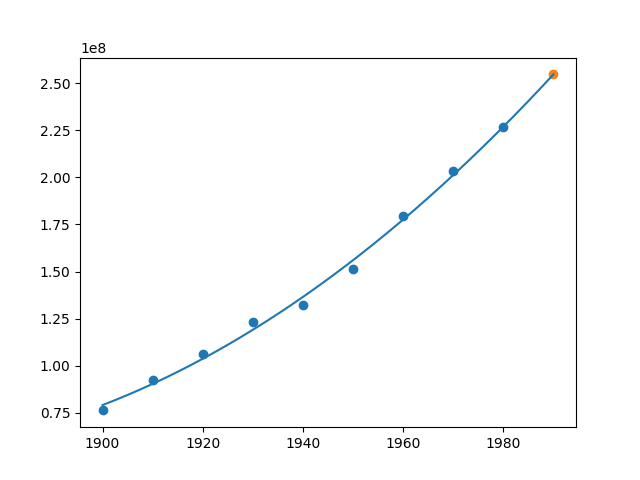
\includegraphics[width=0.8\linewidth]{approx.png}
        \caption{m=2}
    \end{figure}

    m=0 val: 143369177 err: 42.35\% \\
    m=1 val: 235808109 err: 5.19\% \\
    \textbf{m=2 val: 254712944 err: 2.41\%} \\
    m=3 val: 261378612 err: 5.09\%\ \\
    m=4 val: -116331273 err: 146.77\% \\
    m=5 val: 472089589 err: 89.82\% \\
    m=6 val: 1269697652 err: 410.51\% \\
    m=0 AIC = 340.79 \\
    m=1 AIC = 308.83 \\
    \textbf{m=2 AIC = 299.23} \\
    m=3 AIC = 304.66 \\
    m=4 AIC = 400.71 \\
    m=5 AIC = 418.88 \\
    m=6 AIC = 517.97

    \subsection{Zadanie 2.}

\end{document}
